\section{Theorie}
\label{sec:Theorie}

Wird Röntgenstrahlung an Materie gestreut, treten zwei verschiedene Arten von Streuung auf.
Zunächst die zu erwartende inelastische Streuung, allerdings ebenfalls eine elastische inkohärente Streuung.
Dabei wierd beobachtet, dass dieser Teil eine verlängerte Wellenlänge besitzt.
Dem zu Grunde liegt der Compton-Effekt, dieser ist schematisch in \autoref{fig:bild1} dargestellt.

\begin{figure}
    \centering
    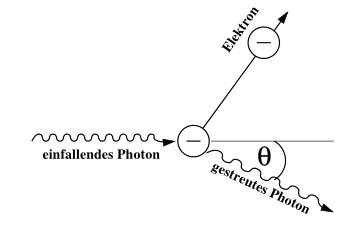
\includegraphics[width=\textwidth/2]{images/bild1.png}
    \caption{Theoretische Funktionsweise des Compton Effekts. \cite{V603}}
    \label{fig:bild1}
\end{figure}

Trifft ein Photon mit der Wellenlänge $\lambda _1$ auf ein Elektron, gibt es einen Teil seiner Energie $E$ ab.
Der Definiton der Energie eines Photons

\begin{equation}
    E = h \cdot f = h \cdot \frac{c}{\lambda}
    \label{eq:energie}
\end{equation}

entsprechend, wird die Wellenlänge des Photons länger.
Dabei ist $h$ das Plancksche Wirkungsquantum und $c$ die Lichtgeschwindigkeit.
Nach dem Stoß besitzt dieses also die Wellenlänge $\lambda _2$.
Das Elektron wird in einem bestimmen Winkel $\theta$ abgelenkt.
Über die Energie- und Impulserhaltung kann die Differenz der beiden Wellenlängen 

\begin{equation}
\Delta \lambda = \lambda _2 - \lambda _1 = \frac{h}{m_\text{e} \cdot c} \cdot \left(1 - \cos{\theta}\right)
    \label{eq:deltalambda}
\end{equation}

bestimmt werden.
Der Vorfaktor  

\begin{equation}
    \lambda _\text{C} = \frac{h}{m_\text{e} \cdot c}
    \label{eq:compton}
\end{equation}

wird Compton-Wellenlänge $\lambda _\text{C}$ genannt und ist je nach Stoßpartnerns des Photons definiert.
In diesem Falle wird durch die Elektronenmasse $m_\text{e}$ die Compton-Wellenlänge eines Elektons betrachtet.

Die verwendete Röntgenstrahlung setzt sich aus dem kontinuierlichen Bremsspektrum und der charakteristischen Röntgenstrahlung zusammensetzt.
Beide Bestandteile entstehen im Zuge des gleichen Prozesses.
Wird eine Glühkathode weit genug erhitzt emittiert sie Elektronen, die sich dann zur Anode hin beschleunigen.
Dort werden sie derart stark abgebremst, dass sie die Bremsstrahlung aussenden. 
Während dieses Prozesses wird ein Photon mit genau dieser verlorenen Energie ausgesendet.
Beim Einschlag des Elektrons in das Atom werden bereits vorhandene Elektronen herausgeschlagen.
Die jetzt leeren Plätze werden von anderen Elektronen aufgefüllt, dabei entsteht die charakteristische Röntgenstrahlung.

Die Röntgenstrahlung wird dabei benutzt um die Compton-Wellenlänge zu bestimmen.
Dringt sie mit einer Intensität $I_0$ durch ein Material hindurch, wird sie nach dem Delamber'schen Gesetz 

\begin{equation}
    I = I_0 \cdot e^{- \mu \cdot d}
    \label{eq:delamber}
\end{equation}

Die Intensität nimmt schneller ab, wenn die Wellenlänge groß ist, spricht die Transmission durch den Körper sinkt.
Zudem wird sie exponentiell von der Dicke $d$ des Materials beeinflusst.
Wichtig ist hier der Absorptionskoeffizent $\mu$, dieser setzt sich aus mehreren anderen Koeffizienten zusammen, unter anderem aus dem Absorptionskoeffizent des Compton-Effekts.

Um die Röntgenstrahlung hinsichtlich ihrer Energie und Wellenlänge zu analysieren wird die Bragg'sche Reflexion verwendet.
Die Photonen werden dabei z.B. auf das Gitter eines LiF-Kristalls gelenkt und dort um den Winkel $\alpha$ gebeugt.
Damit ergibt sich folgender Zusammenhang

\begin{equation}
    2 d \sin{\alpha} = n \cdot \lambda.
    \label{eq:bragg}
\end{equation}
$n$ ist der Brechungsgrad des Kristalls und $d$ hier die Gitterkonstante.
